% Preambel
\documentclass[a4paper,openany]{report}


\usepackage{a4wide}
\usepackage[ansinew]{inputenc}
\usepackage[T1]{fontenc}
\RequirePackage{ifpdf}

\usepackage{hyperref}
	\hypersetup{%
  colorlinks=true,   % activates colored references
  pdfpagemode=None,  % PDF-Viewer starts without content et.al.
  pdfstartview=FitH, % PDF-Viewer uses a defined page width
  %linkbordercolor=111,
  % citebordercolor=111,
  citecolor=blue,
  linkcolor=blue}

\ifpdf
  \usepackage[pdftex]{graphicx}
	  \DeclareGraphicsExtensions{.pdf}
\else
  \usepackage[dvips]{graphicx}
	  \DeclareGraphicsExtensions{.eps}
\fi
	
\usepackage{fancyhdr}
\usepackage{booktabs}
%\usepackage[dvips]{rotating}
\usepackage{multirow}
\usepackage{multicol}

\usepackage{color}
\usepackage{amsmath}
\usepackage{alltt}
%\usepackage{array}
%\usepackage{colortbl}

\clubpenalty = 10000
\widowpenalty = 10000 \displaywidowpenalty = 10000

\definecolor{hellgrau}{gray}{0.95}
\definecolor{dunkelgrau}{gray}{0.55}



\renewcommand{\headrulewidth}{0pt} % no head rule
\renewcommand{\footrulewidth}{0pt} % no foot rule




%\nointend
%%%%%%%%%%%%%%%%%%%%%%%%%%%%%%
% start text here!!



\begin{document}
\pagenumbering{roman}

\title{A neural network toolbox for Octave\\
			Developer's Guide\\
			  Version: 0.1.9}

\author{M. Schmid}
\maketitle


\tableofcontents
\pagenumbering{arabic}

\chapter{Introduction}

\section{Compatibility to Matlab's \texttrademark Neural Network Toolbox}
The compatibility is one of the strongest targets during developing this toolbox.
If I have to develope an incompatibility e.g. in naming the functions, it will be descriped
in this documentation. Even though it should be clear that I can't make a one to one copy.  First,
the m-files are copyrighted and second, octave doesn't yet support the object oriented-programming techonology.\\

If you find a bug, any not described incompatibility or have some suggestions, please write me at
michaelschmid@users.sourceforge.net. This will help improving this toolbox.


\section{Version numbers of the neural network toolbox}

The first number describes the major release. Version number V1.0 will be the first toolbox release which should have the same functions like the Matlab R14 SP3 neural network Toolbox.\\

The second number defines the finished functions. So to start, only the MLPs will realised and so this will be the number V0.1.0.\\

The third number defines the status of the actual development and function. V0.0.1 means no release with MLP, actually, everything under construction... ;-D.\\

Right now it's version V0.1.3 which means MLP works and currently the transfer function logsig is added.

\section{Known incompatibilities}
\label{chap:intro:sec:knownIncompatibilities}


\subsection{Function names}

\subsubsection{minmax}
\textit{minmax} is in this toolbox called \textit{min\_max}. This is because Octave already has
a function whichs name is \textit{minmax}. This is a c file and the functions \textit{min} and \textit{max} are therein realized.





\chapter{Octave}
This chapter describes all functions available in the neural network toolbox in Octave.



\input{octave/functions/isposint_netw_privOct}
\chapter{Coding Guideline}
Some genereal descriptions why a variable has a chosen name. This is valid for the complete
toolbox... or so :-)\\
Here is only the description of variable names, which aren't visible to the user. Visible names are
described in the User's Guide!\\
The variable identifiers are taken from \cite{4}. One difference is purposeful added. If a variable has only one letter, a second small letter will be added to make it searchable. Who has ever tried to search a variable called "t"?

\section{Variable identifier}

\begin{tabbing}
\hspace*{1em} \= \textcolor{blue}{Identifier} \hspace*{3em}\= \textcolor{blue}{Description:} \\ 
  \textbf{Aa} \> \> hold the network values after transfer function.\\
  blf \>  \> \textbf{b}atch \textbf{l}earning \textbf{f}unction \\
  btf  \>  \> \textbf{b}atch \textbf{t}rainings \textbf{f}unction \\
  \textbf{Jj} \>  \> Jacobi matrix \\
  \textbf{Nn}  \> \> hold the network values before transfer function.\\  						
  net	\> \> structure which holds the neural network informations \\
  pf \>  \> \textbf{p}erformance \textbf{f}unction \\
  \textbf{Pp}				\>						\>input matrix; nInputs x nDataSets  \\
  \textbf{Pr}	\>		\> input range, this is a Nx2 matrix, that's why the capitalized P \\
  trf \>  \> \textbf{tr}ansfer \textbf{f}unction \\
  \textbf{Tt} \>  \> target matrix, nTargets x nDataSets\\
  \textbf{ss}	\> \> row vector with numbers of neurons in the layers, for each layer, one entry \\
  \textbf{vE}	\> \> row vector with errors... size depends on network structure. \\
  VV \>  \> Validation structure \\
  \textbf{xx} \>  \> Weight vector in column format\\
  
\end{tabbing}

\subsection{Nn}
\textbf{Nn} is a cell array and has one entry for each layer. In reality, this will have 2 or 3 layers.\\
In \textbf{Nn\{1,1\}} are the values for the first hidden layer. The size of this matrix depends
on the number of neurons used for this layer.\\
In \textbf{Nn\{2,1\}} are the values for the second hidden layer or the output layer. The size of this matrix depends
on the number of neurons used for this layer and so on ...\\
\textbf{Nn\{x,1\}} where \textbf{x} can be $\infty$.\\

\subsection{Aa}
\textbf{Aa} is a cell array and has one entry for each layer.\\
In \textbf{Aa\{1,1\}} are the values for the first hidden layer. The size of this matrix depends
on the number of neurons used for this layer.\\
In \textbf{Aa\{2,1\}} are the values for the second hidden layer or the output layer. The size of this matrix depends
on the number of neurons used for this layer.\\
See \textbf{Nn} for a more detailed description.\\

\subsection{vE}
\textbf{vE} is also a cell array which holds in the last (second) element the error vector. It's not completly clear, why in the last (second) element.\\
The number of rows depends on the number of output neurons. For one output neuron, \textbf{vE} holds only one row, for 2 output neurons, this holds of course 2 rows, and so on. 

\subsection{Jj}
This is the short term for the Jacobi matrix.
\chapter{Algorithm}
Here are some general thoughts about calculating parts are used in algorithm.

\section{Levenberg Marquardt}
This algorithm will be programed with \cite{4}.

\subsection{Sensitivity Matrix}
How does this looks like?\\
\begin{enumerate}
	\item for a 1-1-1 MLP
	\item for a 2-1-1 MLP
	\item for a 1-2-1 MLP
\end{enumerate}

\subsubsection{1-1-1 MLP}
In this case, the MLP holds one input neuron, one hidden neuron and one output neuron. The number of weights needed for this MLP is 4 (2 weights, 2 biases).\\

It needs two sensitivity matrices because the two layers. Each sensitivity matrix will hold 1 element.
This is taken from \cite{4}, example P12.5 page 12-44. Attention, in this example are two data sets used, this is the reason for the 4 elements...!

\subsubsection{2-1-1 MLP}
In this case, the MLP holds two input neurons, one hidden neuron and one output neuron. The number of weights needed for this MLP is 5 (3 weights, 2 biases).\\

It needs also two sensitivity matrices because the two layers. Actually, the input is not only a scalar, it is a vector with 2 elements. Even though, again after \cite{4}. I think the sensitivity matrices will hold only 1 element. So the number of elements will bi proportional to the number of hidden neurons and the number of output neurons.

\subsubsection{1-2-1 MLP}
In this case, the MLP holds one input neuron, two hidden neurons and one output neuron. The number of weights needed for this MLP is 7 (4 weights, 3 biases).\\

It needs also two sensitivity matrices because the two layers. Actually, the input is again only a scalar. 
Now calculating $n_1^1$ will result in a row vector with 2 elements. $n_1^2$ will hold only one element and so we have 3 elements in the sensitivity matrix.\\

We can say, the number of hidden neurons is responsible for the dimension of the sensitivity matrices.
For example, a 4-3-1 MLP with 100 data sets will generate following sensitivity matrix for the first layer:
$\tilde{\textbf{S}}^1 = [\tilde{\textbf{S}}^1_1 | \tilde{\textbf{S}}^1_2 | ... | \tilde{\textbf{S}}^1_{100}]$\\
\noindent $\tilde{\textbf{S}}^1_1$ will hold 3 elements  $\tilde{\textbf{S}}^1_1 = [\tilde{\textbf{S}}^1_{1,1} ~ \tilde{\textbf{S}}^1_{2,1} ~ \tilde{\textbf{S}}^1_{3,1}]^T$;
$\tilde{\textbf{S}}^1_2 = [\tilde{\textbf{S}}^1_{1,2} ~ \tilde{\textbf{S}}^1_{2,2} ~ \tilde{\textbf{S}}^1_{3,2}]^T$ and so on. So matrix will have a size of 3x100 for $\tilde{\textbf{S}}^1_{1}$
and a size of 1x100 for $\tilde{\textbf{S}}^1_{2}$.\\

By the way, the jacobian matrix will be a 100x20 matrix ..






\chapter{Test}

\section{isposint}
\begin{verbatim}
%!shared
%! disp("testing isposint")
%!assert(isposint(1)) # this should pass
%!assert(isposint(0.5),0) # should return zero
%!assert(isposint(-1),0) # should return zero
%!assert(isposint(-1.5),0) # should return zero
%!assert(isposint(0),0) # should return zero
%!fail("isposint([0 0])","Input argument must not be a vector, only scalars are allowed!")
%!fail("isposint('testString')","Input argument must not be a vector, only scalars are allowed!")
\end{verbatim}

\section{min\_max}
\subsection{min\_max}
Checks for minimal and maximal values of an input matrix for \textbf{newff}.\\

\subsubsection{Syntax:}

$pr = min\_max(mInputs)$\\

\subsubsection{Description:}
\textit{mInputs} must be a matrix with input training data sets. This means in the case, for a 9-2-1 MLP
(this means 9 input-, 2 hidden- and 1 output-neuron) with 100 input training data sets, the matrix must be
an 9x100 matrix. \textit{pr} will then be a 9x2 matrix with minimal values in the first column and maximal values in the second column. If a row holds 2 zeros, a warning will appear (no information in this row!).

\subsubsection{Important:}
The equival function in MATLAB(TM) is called \textit{minmax}. This is not possible because the functions \textit{min} and \textit{max} in Octave are programed in minmax.cc!
\section{newff}
\subsection{min\_max}
Checks for minimal and maximal values of an input matrix for \textbf{newff}.\\

\subsubsection{Syntax:}

$pr = min\_max(mInputs)$\\

\subsubsection{Description:}
\textit{mInputs} must be a matrix with input training data sets. This means in the case, for a 9-2-1 MLP
(this means 9 input-, 2 hidden- and 1 output-neuron) with 100 input training data sets, the matrix must be
an 9x100 matrix. \textit{pr} will then be a 9x2 matrix with minimal values in the first column and maximal values in the second column. If a row holds 2 zeros, a warning will appear (no information in this row!).

\subsubsection{Important:}
The equival function in MATLAB(TM) is called \textit{minmax}. This is not possible because the functions \textit{min} and \textit{max} in Octave are programed in minmax.cc!
\section{prestd}
\subsection{min\_max}
Checks for minimal and maximal values of an input matrix for \textbf{newff}.\\

\subsubsection{Syntax:}

$pr = min\_max(mInputs)$\\

\subsubsection{Description:}
\textit{mInputs} must be a matrix with input training data sets. This means in the case, for a 9-2-1 MLP
(this means 9 input-, 2 hidden- and 1 output-neuron) with 100 input training data sets, the matrix must be
an 9x100 matrix. \textit{pr} will then be a 9x2 matrix with minimal values in the first column and maximal values in the second column. If a row holds 2 zeros, a warning will appear (no information in this row!).

\subsubsection{Important:}
The equival function in MATLAB(TM) is called \textit{minmax}. This is not possible because the functions \textit{min} and \textit{max} in Octave are programed in minmax.cc!
\section{purelin}
\subsection{purelin}

\begin{figure}[htb]
\centering
  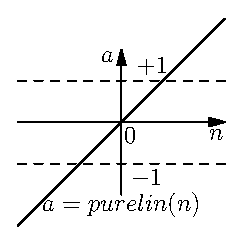
\includegraphics{octave/neuroPackage/graphics/purelin}
\caption{Linear transfer function}
\label{fig:purelinTransferFunction}
\end{figure}

\begin{figure}[htb]
\centering
  
\includegraphics{octave/neuroPackage/graphics/purelinlogo}
\caption{Linear transfer function logo}
\label{fig:purelinTransferFunctionLogo}
\end{figure}


\section{subset}
\subsection{subset}

\textit{subset} can be used to optimize the data sets for train, test and validation of a neural
network.\\

\noindent \textbf{\textcolor{brown}{Syntax:}}\\

\noindent [mTrain, mTest, mVali] = subset(mData,nTargets,iOpti,fTest,fVali);\\

\noindent \textbf{\textcolor{brown}{Description:}}\\

\noindent  \textbf{Left-Hand-Side:}\\
\noindent mTrain: (R+T) x M matrix with R input rows, T output rows and M columns
				where M <= N.\\
\noindent mTest:  (R+T) x S matrix with R input rows, T output rows and S columns
				where S <= N.\\
\noindent mVali:  (R+T) x U matrix with R input rows, T output rows and U columns
				where U <= N. And U can only exist, if S also exist.\\

\noindent  \textbf{Right-Hand-Side:}\\
\noindent mData: (R+T) x N matrix with R input rows, T output rows and N columns\\ 
\noindent nTargets: Number of T output rows\\ 
\noindent iOpti: Integer value to define level of optimization.\\
\noindent fTest: Fraction to define the percentage of data sets which should be used for testing. \\
\noindent fVali: Fraction to define the percentage of data sets which should be used for testing.\\

\noindent iOpti can have following values:\\
0	: no optimization\\
1	: will randomise the column order and rerange the columns containing min and max values to be in the train set\\
2	:	will NOT randomise the column order, but rerange the columns containing min and max values to be in the train set\\

\noindent fTest or fValie have following meaning:\\
Each of this arguments can be a fraction or zero. The value 1 is not allowed! The sum of both values
must also be smaller than 1!\\
Example: fTest = 1/3\\

\noindent \textbf{Default values}\\
\noindent iOpti		= 1\\
\noindent fTest		= 1/3\\
\noindent fVali		= 1/6\\

\noindent \textbf{\textcolor{brown}{Examples:}}\\

\noindent mTrain = subset(mData,2,1,0,0)\\
\noindent [mTrain,mTest] = subset(mData,2,1,1/3,0);\\
\noindent [mTrain,mTest,mVali] = subset(mData,1);\\
\noindent [mTrain,mTest,mVali] = subset(mData,1,1,1/3,1/6);\\
\section{\_\_analyzerows}
\begin{verbatim}
%!shared b, retmat
%! disp("testing __analyzerows")
%! b = [1 0 0 1; 1 0 0 0; 1 2 0 1];
%! retmat = __analyzerows(b);
%!assert(retmat(1,1)==1);#%!assert(retmat(1,1)==1);
%!assert(retmat(2,1)==1);
%!assert(retmat(3,1)==0);
%! b = [1 0 0 2; 1 0 0 0; 1 1 1 1];
%! retmat = __analyzerows(b);
%!assert(retmat(1,2)==0);
%!assert(retmat(2,2)==0);
%!assert(retmat(3,2)==1);
%! b = [1 0 0 2; 1 0 0 0; 1 1 1 1];
%! retmat = __analyzerows(b);
%!assert(retmat(1,3)==2);
%!assert(retmat(2,3)==0);
%!assert(retmat(3,3)==0);
%! retmat = __analyzerows(b);
%!assert(retmat(1,4)==1);
%!assert(retmat(2,4)==0);
%!assert(retmat(3,4)==0);
\end{verbatim}

\section{\_\_copycoltopos1}
\begin{verbatim}
%!shared a, retmat
%! disp("testing __copycoltopos1")
%! a = [0 1 2 3 4; 5 6 7 8 9];
%! retmat = __copycoltopos1(a,3);
%!assert(retmat(1,1)==2);
%!assert(retmat(2,1)==7);
%! retmat = __copycoltopos1(a,5);
%!assert(retmat(1,1)==4);
%!assert(retmat(2,1)==9);
\end{verbatim}

\section{\_\_optimizedatasets}
\begin{verbatim}
%!shared retmatrix, matrix
%! disp("testing __optimizedatasets")
%! matrix = [1 2 3 2 1 2 3 0 5 4 3 2 2 2 2 2 2; \
%!			 0 1 1 0 0 0 0 0 0 0 0 0 0 0 1 1 0; \
%!			-1 3 2 4 9 1 1 1 1 1 9 1 1 1 9 9 0; \
%!			 2 3 2 3 2 2 2 2 3 3 3 3 1 1 1 1 1];
%! ## The last row is equal to the neural network targets
%! retmatrix = __optimizedatasets(matrix,9,1);
%! ## the above statement can't be tested with assert!
%! ## it contains random values! So pass a "success" message
%!assert(1==1);
%! matrix = [1 2 3 2 1 2 3 0 5 4 3 2 2 2 2 2 2; \
%!			 0 1 1 0 0 0 0 0 0 0 0 0 0 0 1 1 0; \
%!			-1 3 2 4 9 1 1 1 1 1 9 1 1 1 9 9 0; \
%!			 2 3 2 3 2 2 2 2 3 3 3 3 1 1 1 1 1];
%! ## The last row is equal to the neural network targets
%! retmatrix = __optimizedatasets(matrix,9,1,0);
%!assert(retmatrix(1,1)==5);
%!assert(retmatrix(2,1)==0);
%!assert(retmatrix(3,1)==1);
%!assert(retmatrix(4,1)==3);
\end{verbatim}

\section{\_\_randomisecols}
\begin{verbatim}
%!# no test possible, contains randperm which is using
%!# some randome functions
\end{verbatim}

\section{\_\_rerangecolumns}
\begin{verbatim}
%!shared matrix,analyzeMatrix,nTrainSets, returnmatrix
%! disp("testing __rerangecolumns")
%! matrix = [0 1 0 0 0 0 1 0 1 1;  \
%!			 4 4 4 4 4 4 4 4 4 4;  \
%!        -1.1 -1.1 2 3 4 3.2 1 8 9 10; \
%!           0 1.1 3 4 5 2 10 10 2 3; \
%!          -1 1 1 1 1 2 3 4 1 5];
%! analyzeMatrix = [1 0 0 0; 0 1 0 0; 0 0 2 1; 0 0 1 2; 0 0 1 1];
%! nTrainSets = 8;
%! returnmatrix = __rerangecolumns(matrix,analyzeMatrix,nTrainSets);
%!assert(returnmatrix(1,1)==1);
%!assert(returnmatrix(2,1)==4);
%!assert(returnmatrix(3,1)==1);
%!assert(returnmatrix(4,1)==10);
%!assert(returnmatrix(5,1)==3);
%! matrix = [0 1 0 0 0 0 1 0 1 1; 			\
%!			 4 4 4 4 4 4 4 4 4 4; 			\
%!          -1.1 -1.1 2 3 4 3.2 1 8 9 10; 	\
%!           0 1.1 3 4 5 2 10 10 2 3; 		\
%!          -1 1 1 1 1 2 3 4 1 5;     		\
%!			 0 1 2 1 2 1 2 3 4 5;];  # the last row is euqal to the nnet targets
%! analyzeMatrix = [1 0 0 0; 0 1 0 0; 0 0 2 1; 0 0 1 2; 0 0 1 1];
%! nTrainSets = 8;
%! returnmatrix = __rerangecolumns(matrix,analyzeMatrix,nTrainSets);
%!assert(returnmatrix(1,1)==1);
%!assert(returnmatrix(2,1)==4);
%!assert(returnmatrix(3,1)==1);
%!assert(returnmatrix(4,1)==10);
%!assert(returnmatrix(5,1)==3);
%!assert(returnmatrix(6,1)==2);
\end{verbatim}


\chapter{analyzing matlab functions}

\section{analyzing newff}
First, \textit{newff} will be analyzed for a X-X-X mlp. This means, maximum 3 layers, including the input layer. Or in words, one input- one hidden- and one output-layer. The number of neurons are choosable.

Following command will be used, to create a new feed-forward neural network:\\
\noindent MLPnet = newff(mMinMaxElements,[nHiddenNeurons nOutputNeurons],...\newline
\{'tansig','purelin'\},'trainlm','learngdm','mse');\\

newff is the matlab command, mMinMaxElements is a $Rx2$-Matrix with minimum and maximum values of the inputs. $R$ is equal to the number of input neurons. [nHiddenNeurons nOutputNeurons] are the scalar values, to define the number of neurons in the hidden and output layer. One value, for each layer. \{'tansig','purelin'\} are the transfer functions, for each layer. This means, 'tansig' for the hidden layer and 'purelin' for the output layer. 'trainlm' is the training algorithm, in this case, Levenberg-Marquardt. 'learngdm' is the learn algorithm and 'mse' is the performance function, \textbf{m}ean-\textbf{s}quare-\textbf{e}rror.\\
MLPnet will be a structure with following content:

\begin{verbatim}
Neural Network object:

    architecture:

         numInputs: 1
         numLayers: 2
       biasConnect: [1; 1]
      inputConnect: [1; 0]
      layerConnect: [0 0; 1 0]
     outputConnect: [0 1]
     targetConnect: [0 1]

        numOutputs: 1  (read-only)
        numTargets: 1  (read-only)
    numInputDelays: 0  (read-only)
    numLayerDelays: 0  (read-only)

    subobject structures:

            inputs: {1x1 cell} of inputs
            layers: {2x1 cell} of layers
           outputs: {1x2 cell} containing 1 output
           targets: {1x2 cell} containing 1 target
            biases: {2x1 cell} containing 2 biases
      inputWeights: {2x1 cell} containing 1 input weight
      layerWeights: {2x2 cell} containing 1 layer weight

    functions:

          adaptFcn: 'trains'
           initFcn: 'initlay'
        performFcn: 'mse'
          trainFcn: 'trainlm'

    parameters:

        adaptParam: .passes
         initParam: (none)
      performParam: (none)
        trainParam: .epochs, .goal, .max_fail, .mem_reduc, 
                    .min_grad, .mu, .mu_dec, .mu_inc, 
                    .mu_max, .show, .time

    weight and bias values:

                IW: {2x1 cell} containing 1 input weight matrix
                LW: {2x2 cell} containing 1 layer weight matrix
                 b: {2x1 cell} containing 2 bias vectors

    other:

          userdata: (user stuff)
\end{verbatim}
\textit{numInputs: 1}: one input layer\\
\noindent \textit{numLayers: 2}: one hidden and one output layer\\
\noindent \textit{biasConnect: [1; 1]}: unknown till now!!\\
\noindent \textit{inputConnect: [1; 0]}: unknown till now!!\\
\noindent \textit{layerConnect: [0 0; 1 0]}: unknown till now!!\\
\noindent \textit{outputConnect: [0 1]}: unknown till now!!\\
\noindent \textit{targetConnect: [0 1]}: unknown till now!!\\
\noindent \textit{numOutputs: 1  (read-only)}: unknown till now!!\\
\noindent \textit{numTargets: 1  (read-only)}: unknown till now!!\\
\noindent \textit{numInputDelays: 0  (read-only)}: unknown till now!!\\
\noindent \textit{numLayerDelays: 0  (read-only)}: unknown till now!!\\
\noindent \textit{inputs: {1x1 cell} of inputs}: input layer definition\\
Because we have defined only one input layer, you can see the detailed definition with
following command in the matlab prompt:\\
\begin{verbatim}
	MLPnet.inputs{1}

ans = 

       range: [26x2 double]
        size: 26
    userdata: [1x1 struct]
\end{verbatim}
range are the min. and max. values of the inputs. size is the number of input neurons and userdata are user specified inputs...!\\
\noindent \textit{layers: {2x1 cell} of layers}: hidden and output layer definition\\
The dimension of $2x1 cell$ is because we have one hidden and one output layer. So too see the details of the hidden layer definitions, we have to enter:
\begin{verbatim}
K>> MLPnet.layers{1}

ans = 

     dimensions: 2
    distanceFcn: ''
      distances: []
        initFcn: 'initnw'
    netInputFcn: 'netsum'
      positions: [0 1]
           size: 2
    topologyFcn: 'hextop'
    transferFcn: 'tansig'
       userdata: [1x1 struct]
\end{verbatim}
and for the output layer:
\begin{verbatim}
K>> MLPnet.layers{2}

ans = 

     dimensions: 1
    distanceFcn: ''
      distances: []
        initFcn: 'initnw'
    netInputFcn: 'netsum'
      positions: 0
           size: 1
    topologyFcn: 'hextop'
    transferFcn: 'purelin'
       userdata: [1x1 struct]
\end{verbatim}

\noindent \textit{outputs: {1x2 cell} containing 1 output}: output layer definitions\\
\begin{verbatim}
K>> MLPnet.outputs

ans = 

     []    [1x1 struct]
\end{verbatim}
How knows, why this is a $1x2 cell$? The next command will also show the detailed definition! Of course, realy simple.
\begin{verbatim}
K>> MLPnet.outputs{2}

ans = 

        size: 1
    userdata: [1x1 struct]
\end{verbatim} 

\noindent \textit{targets: {1x2 cell} containing 1 target}: unknow till now\\

\noindent \textit{biases: {2x1 cell} containing 2 biases}: detailed definitions, for the biases\\
\begin{verbatim}
K>> MLPnet.biases

ans = 

    [1x1 struct]
    [1x1 struct]

K>> MLPnet.biases{1}

ans = 

       initFcn: ''
         learn: 1
      learnFcn: 'learngdm'
    learnParam: [1x1 struct]
          size: 2
      userdata: [1x1 struct]

K>> MLPnet.biases{2}

ans = 

       initFcn: ''
         learn: 1
      learnFcn: 'learngdm'
    learnParam: [1x1 struct]
          size: 1
      userdata: [1x1 struct]
\end{verbatim}
      inputWeights: {2x1 cell} containing 1 input weight
      layerWeights: {2x2 cell} containing 1 layer weight


\paragraph{weight and bias values:}

\subparagraph{IW:}
\begin{verbatim}
K>> MLPnet.IW

ans = 

    [2x26 double]
               []
\end{verbatim}

\subparagraph{LW:}
\begin{verbatim}
K>> MLPnet.LW

ans = 

              []     []
    [1x2 double]     []
\end{verbatim}

\subparagraph{b:}
\begin{verbatim}
K>> MLPnet.b

ans = 

    [2x1 double]
    [   -0.3908]
\end{verbatim}


\paragraph{net.trainParam:}
Output for the Levenberg-Marquardt train algorithm.
\begin{verbatim}
K>> MLPnet.trainParam

ans = 

       epochs: 100
         goal: 0
     max_fail: 5
    mem_reduc: 1
     min_grad: 1.0000e-010
           mu: 0.0010
       mu_dec: 0.1000
       mu_inc: 10
       mu_max: 1.0000e+010
         show: 25
         time: Inf
\end{verbatim}
\section{analyzing newp}


Following command will be used, to create a new neural perceptron:\\
\noindent net = newfp(mMinMaxElements,nNeurons);\\

newp is the matlab command, mMinMaxElements is a $Rx2$-Matrix with minimum and maximum values of the inputs. $R$ is equal to the number of input neurons. \\

net = newp([0 1; -2 2],1)

\begin{verbatim}
net =

    Neural Network object:

    architecture:

         numInputs: 1
         numLayers: 1
       biasConnect: [1]
      inputConnect: [1]
      layerConnect: [0]
     outputConnect: [1]
     targetConnect: [1]

        numOutputs: 1  (read-only)
        numTargets: 1  (read-only)
    numInputDelays: 0  (read-only)
    numLayerDelays: 0  (read-only)

    subobject structures:

            inputs: {1x1 cell} of inputs
            layers: {1x1 cell} of layers
           outputs: {1x1 cell} containing 1 output
           targets: {1x1 cell} containing 1 target
            biases: {1x1 cell} containing 1 bias
      inputWeights: {1x1 cell} containing 1 input weight
      layerWeights: {1x1 cell} containing no layer weights

    functions:

          adaptFcn: 'trains'
           initFcn: 'initlay'
        performFcn: 'mae'
          trainFcn: 'trainc'

    parameters:

        adaptParam: .passes
         initParam: (none)
      performParam: (none)
        trainParam: .epochs, .goal, .show, .time

    weight and bias values:

                IW: {1x1 cell} containing 1 input weight matrix
                LW: {1x1 cell} containing no layer weight matrices
                 b: {1x1 cell} containing 1 bias vector

    other:

          userdata: (user stuff)
\end{verbatim}
\textit{numInputs: 1}: one input layer\\
\noindent \textit{numLayers: 1}: one output layer\\
\noindent \textit{biasConnect: [1]}: unknown till now!!\\
\noindent \textit{inputConnect: [1]}: unknown till now!!\\
\noindent \textit{layerConnect: [0]}: unknown till now!!\\
\noindent \textit{outputConnect: [1]}: unknown till now!!\\
\noindent \textit{targetConnect: [1]}: unknown till now!!\\
\noindent \textit{numOutputs: 1  (read-only)}: unknown till now!!\\
\noindent \textit{numTargets: 1  (read-only)}: unknown till now!!\\
\noindent \textit{numInputDelays: 0  (read-only)}: unknown till now!!\\
\noindent \textit{numLayerDelays: 0  (read-only)}: unknown till now!!\\
\noindent \textit{inputs: {1x1 cell} of inputs}: input layer definition\\
Because we have defined only one input layer, you can see the detailed definition with
following command in the matlab prompt:\\
\begin{verbatim}
>> net.inputs{1}

ans =

       range: [2x2 double]
        size: 2
    userdata: [1x1 struct]
    
net.inputs{1}.range

ans =

     0     1
    -2     2
    
net.inputs{1}.size

ans =

     2
     
net.inputs{1}.userdata

ans =

    note: 'Put your custom input information here.'
\end{verbatim}
range are the min. and max. values of the inputs. size is the number of input neurons and userdata are user specified inputs...!\\
\noindent \textit{layers: {1x1 cell} of layers}: actually no idea what's inside this cell!!!\\
To see the details of this layer definition, we have to enter:
\begin{verbatim}
net.layers{1}

ans = 

     dimensions: 1
    distanceFcn: ''
      distances: []
        initFcn: 'initwb'
    netInputFcn: 'netsum'
      positions: 0
           size: 1
    topologyFcn: 'hextop'
    transferFcn: 'hardlim'
       userdata: [1x1 struct]
\end{verbatim}
and for the output layer:
\begin{verbatim}
net.outputs{1}

ans = 

        size: 1
    userdata: [1x1 struct]
\end{verbatim}

\begin{verbatim}
 net.outputs{1}.userdata

ans = 

    note: 'Put your custom output information here.'
\end{verbatim}

\begin{verbatim}
net.targets

ans = 

    [1x1 struct]
\end{verbatim}

\begin{verbatim}
net.targets{1}

ans =

        size: 1
    userdata: [1x1 struct]
\end{verbatim}

\begin{verbatim}
net.targets{1}.userdata

ans = 

    note: 'Put your custom output information here.'
\end{verbatim}

\begin{verbatim}
net.biases{1}

ans =

       initFcn: 'initzero'
         learn: 1
      learnFcn: 'learnp'
    learnParam: []
          size: 1
      userdata: [1x1 struct]
\end{verbatim}


\begin{verbatim}
net.biases{1}.userdata

ans =

    note: 'Put your custom bias information here.'
\end{verbatim}


\begin{verbatim}
net.inputWeights

ans = 

    [1x1 struct]
\end{verbatim}


\begin{verbatim}
net.inputWeights{1}

ans = 

        delays: 0
       initFcn: 'initzero'
         learn: 1
      learnFcn: 'learnp'
    learnParam: []
          size: [1 2]
      userdata: [1x1 struct]
     weightFcn: 'dotprod'
\end{verbatim}

\begin{verbatim}
net.layerWeights

ans = 

    {[]}
\end{verbatim}

\begin{verbatim}
net.LW

ans = 

    {[]}
\end{verbatim}

\begin{verbatim}
net.IW

ans = 

    [1x2 double]
\end{verbatim}

\begin{verbatim}
net.IW{1}

ans =

     0     0
\end{verbatim}

\begin{verbatim}
net.b

ans = 

    [0]
\end{verbatim}



\appendix
\chapter{Examples}


\section{Example 1}

This MLP is designed with 2-2-1. This is not a complete example but it will help to understand the
dimensions of all matrices and vectores are used inside the Levenberg-Marquardt algorithm.

\subsection{Data matrices}
The input matrix will be defined like in equation \eqref{equ:mInput} and the output matrix like in 
equation \eqref{equ:mOutput}.

\begin{equation}
  mInput = \left[ \begin{array}{c c c c}
												1 & 2 & 3 & 1   \\
												1	& 1 & 1 & 2 	\\
												1 & 2 & 1 & 2		\\																					
												\end{array}
					\right]
		\label{equ:mInput}
\end{equation}

\begin{equation}
  mOutput = \left[ \begin{array}{c c c c}
												1 & 1.5 & 2 & 3   \\																					
									 \end{array}
					\right]
		\label{equ:mOutput}
\end{equation}




\subsection{Weight matrices}
The first layer matrix will hold 2x3 weights. The second layer matrix will hold 1x2 weights.
The first bias holds 3x1 weights and the second holds only a scalar element.

\subsection{Sensitivity Matrices}
This part is right now not so clear in my mind. What is the dimension of these two matrices?
The first layer sensitivity matrix should be about 2x71. Number of hidden neurons in the rows and number of train data sets in the columns.\\

In the actual version, the dimension is about 71x71 .. so it seems to have a mistake inside the algorithm :-(


% Preamble

%\documentclass[a4paper]{report}

%\usepackage[ngerman]{babel}
%\usepackage[T1]{fontenc}
%\usepackage[ansinew]{inputenc}


%%%%%%%%%%%%%%%%%%%%%%%%%%%%%%
% start text here!!

%\begin{document}

\begin{thebibliography}{XXXXXXX}

\bibitem [1]{1} John W. Eaton

GNU Octave Manual, Edition 3, PDF-Version, February 1997

\bibitem [2]{2} The MathWorks, Inc.

MATLAB Help, MATLAB Version 7.1 (R14SP3), Neural Network Toolbox Version 4.0.6 (R14SP3) 

\bibitem [3]{3} Christopher M. Bishop

Neural Networks for Pattern Recognition, OXFORD University Press, Great Clarendon Streed, Oxford OX2 6DP,
ISBN 0-19-853864-2, 2002

\bibitem [4]{4} Martin T. Hagen, Howard B. Demuth, Mark H. Beale

NEURAL NETWORK DESIGN, PWS Publishing Company, 20 Park Plaza, Boston, MA 02116-4324, ISBN 053494332-2, 1996

\end{thebibliography}
%\end{document}



\end{document}


